% Options for packages loaded elsewhere
\PassOptionsToPackage{unicode}{hyperref}
\PassOptionsToPackage{hyphens}{url}
%
\documentclass[
]{article}
\author{}
\date{\vspace{-2.5em}}

\usepackage{amsmath,amssymb}
\usepackage{lmodern}
\usepackage{iftex}
\ifPDFTeX
  \usepackage[T1]{fontenc}
  \usepackage[utf8]{inputenc}
  \usepackage{textcomp} % provide euro and other symbols
\else % if luatex or xetex
  \usepackage{unicode-math}
  \defaultfontfeatures{Scale=MatchLowercase}
  \defaultfontfeatures[\rmfamily]{Ligatures=TeX,Scale=1}
\fi
% Use upquote if available, for straight quotes in verbatim environments
\IfFileExists{upquote.sty}{\usepackage{upquote}}{}
\IfFileExists{microtype.sty}{% use microtype if available
  \usepackage[]{microtype}
  \UseMicrotypeSet[protrusion]{basicmath} % disable protrusion for tt fonts
}{}
\makeatletter
\@ifundefined{KOMAClassName}{% if non-KOMA class
  \IfFileExists{parskip.sty}{%
    \usepackage{parskip}
  }{% else
    \setlength{\parindent}{0pt}
    \setlength{\parskip}{6pt plus 2pt minus 1pt}}
}{% if KOMA class
  \KOMAoptions{parskip=half}}
\makeatother
\usepackage{xcolor}
\IfFileExists{xurl.sty}{\usepackage{xurl}}{} % add URL line breaks if available
\IfFileExists{bookmark.sty}{\usepackage{bookmark}}{\usepackage{hyperref}}
\hypersetup{
  hidelinks,
  pdfcreator={LaTeX via pandoc}}
\urlstyle{same} % disable monospaced font for URLs
\usepackage[margin=1in]{geometry}
\usepackage{longtable,booktabs,array}
\usepackage{calc} % for calculating minipage widths
% Correct order of tables after \paragraph or \subparagraph
\usepackage{etoolbox}
\makeatletter
\patchcmd\longtable{\par}{\if@noskipsec\mbox{}\fi\par}{}{}
\makeatother
% Allow footnotes in longtable head/foot
\IfFileExists{footnotehyper.sty}{\usepackage{footnotehyper}}{\usepackage{footnote}}
\makesavenoteenv{longtable}
\usepackage{graphicx}
\makeatletter
\def\maxwidth{\ifdim\Gin@nat@width>\linewidth\linewidth\else\Gin@nat@width\fi}
\def\maxheight{\ifdim\Gin@nat@height>\textheight\textheight\else\Gin@nat@height\fi}
\makeatother
% Scale images if necessary, so that they will not overflow the page
% margins by default, and it is still possible to overwrite the defaults
% using explicit options in \includegraphics[width, height, ...]{}
\setkeys{Gin}{width=\maxwidth,height=\maxheight,keepaspectratio}
% Set default figure placement to htbp
\makeatletter
\def\fps@figure{htbp}
\makeatother
\setlength{\emergencystretch}{3em} % prevent overfull lines
\providecommand{\tightlist}{%
  \setlength{\itemsep}{0pt}\setlength{\parskip}{0pt}}
\setcounter{secnumdepth}{-\maxdimen} % remove section numbering
\newlength{\cslhangindent}
\setlength{\cslhangindent}{1.5em}
\newlength{\csllabelwidth}
\setlength{\csllabelwidth}{3em}
\newlength{\cslentryspacingunit} % times entry-spacing
\setlength{\cslentryspacingunit}{\parskip}
\newenvironment{CSLReferences}[2] % #1 hanging-ident, #2 entry spacing
 {% don't indent paragraphs
  \setlength{\parindent}{0pt}
  % turn on hanging indent if param 1 is 1
  \ifodd #1
  \let\oldpar\par
  \def\par{\hangindent=\cslhangindent\oldpar}
  \fi
  % set entry spacing
  \setlength{\parskip}{#2\cslentryspacingunit}
 }%
 {}
\usepackage{calc}
\newcommand{\CSLBlock}[1]{#1\hfill\break}
\newcommand{\CSLLeftMargin}[1]{\parbox[t]{\csllabelwidth}{#1}}
\newcommand{\CSLRightInline}[1]{\parbox[t]{\linewidth - \csllabelwidth}{#1}\break}
\newcommand{\CSLIndent}[1]{\hspace{\cslhangindent}#1}
\ifLuaTeX
  \usepackage{selnolig}  % disable illegal ligatures
\fi

\begin{document}

%\begin{titlepage}
\begin{center}
\huge{\textbf{COVENTRY}}\\
\huge{\textbf{UNIVERSITY}}\\
\vspace*{1\baselineskip}
\Large{\textbf{Faculty of Engineering, Environment and Computing
School of Computing, Electronics and Mathematics}}\\

\vspace*{3\baselineskip}
\Large{MSc. Data Science and Computational Intelligence}\\
\normalsize{7151CEM}\\
\normalsize{\textbf{Computing Individual Research Project}}\\
\vspace*{6\baselineskip}
\LARGE{\textbf{Diabetic Retinopathy Detection Using Deep Learning}}\\
\vspace*{3\baselineskip}

\begin{left}
\Large{Author :{\textbf { Aleena Alby}}}\\
\Large{SID :{\textbf { 11865340}}}\\
\Large{1st Supervisor :{\textbf { Prof. James Brusey}}}\\
\Large{2nd Supervisor :{\textbf { Prof. Fei He}}}\\
\vspace*{1\baselineskip}
\end{left}
\vspace*{8\baselineskip}
\normalsize{Submitted in partial fulfilment of the requirements for the Degree of Master of Science in Data Science and Computational Intelligence}\\
\Large{\textbf{Academic Year: 2022/23}}\\
\end{center}
% \end{titlepage}



\newpage

\newpage

\textbf{Declaration of Originality}

I declare that this project is all my own work and has not been copied
in part or in whole from any other source except where duly
acknowledged. As such, all use of previously published work (from books,
journals, magazines, internet etc.) has been acknowledged by citation
within the main report to an item in the References or Bibliography
lists. I also agree that an electronic copy of this project may be
stored and used for the purposes of plagiarism prevention and detection.

\textbf{Statement of copyright}

I acknowledge that the copyright of this project report, and any product
developed as part of the project, belong to Coventry University.
Support, including funding, is available to commercialise products and
services developed by staff and students. Any revenue that is generated
is split with the inventor/s of the product or service. For further
information please see
\href{http://www.coventry.ac.uk/ipr}{www.coventry.ac.uk/ipr} or contact
\href{mailto:ipr@coventry.ac.uk}{\nolinkurl{ipr@coventry.ac.uk}}.

\textbf{Statement of ethical engagement}

I declare that a proposal for this project has been submitted to the
Coventry University ethics monitoring website
(\url{https://ethics.coventry.ac.uk/}) and that the application number
is listed below (Note: Projects without an ethical application number
will be rejected for marking)

\[Signed:\]\{AleenaAlby\} \underline{Date:}

Please complete all fields.

\begin{longtable}[]{@{}
  >{\raggedright\arraybackslash}p{(\columnwidth - 0\tabcolsep) * \real{0.75}}@{}}
\toprule
\begin{minipage}[b]{\linewidth}\raggedright
First Name: Aleena
\end{minipage} \\
\midrule
\endhead
Last Name: Alby \\
Student ID number \\
Ethics Application Number \\
1\textsuperscript{st} Supervisor Name Prof James Brusey \\
2\textsuperscript{nd} Supervisor Name \\
\bottomrule
\end{longtable}

\pagebreak
\tableofcontents
\pagebreak
\listoftables
\pagebreak
\listoffigures 
\pagebreak

\hypertarget{introduction}{%
\section{Introduction}\label{introduction}}

One of the major causes of eye vision loss is diabetes. While delayed
examination would have a higher effect on the retinal area of the eye,
early detection of diabetes is crucial. The key factors affecting the
rise in the occurrence of this disease are people's lifestyles and other
contributing factors, and it is anticipated that this trend will
continue. According to Tien Y Wong et al, among the 285 million
diabetics worldwide, 33 percent of those individuals exhibit DR
symptoms(\protect\hyperlink{ref-r2015}{R, Ty, and C 2015}). Nearly 90\%
of individuals can be diagnosed, and long-term effects can be reduced,
with thorough screening and regular checkups. The significant issue here
is that DR is primarily an asymptomatic eye condition that does not
manifest distinctive symptoms until a late stage is reached. The manual
examination of retinal image features is a challenging and taxing task,
nevertheless. Many automated diagnostic technologies have been created
recently to help ophthalmologists examine retinal abnormalities, which
has helped to solve this problem.

\hypertarget{background-to-the-project}{%
\subsection{Background to the Project}\label{background-to-the-project}}

\hypertarget{project-objectives}{%
\subsection{Project Objectives}\label{project-objectives}}

Can DL outperform other methods such as SVM, Logistic Regression,
Decision Tree in producing a high performing classifier for DR on unseen
data?

\hypertarget{overview-of-this-report}{%
\subsection{Overview of This Report}\label{overview-of-this-report}}

\newpage

\hypertarget{literature-review}{%
\section{Literature Review}\label{literature-review}}

In recent years, numerous deep learning based automatic DR detection
systems have emerged. In this section, some of the recent research
projects have been addressed.

Using transfer learning, Esra Kaya and Ismail Saritas created CNN for
the identification of diabetic retinopathy
(\protect\hyperlink{ref-9828576}{Kaya and Saritas 2022}). They utilised
the DRIVE dataset (Digital Retinal Images for Vessel Extraction). They
utilised contrast-limited adaptive histogram equalisation to improve the
clarity of the image. They assessed the ResNet18, GoogleNet, and
SqueezeNet CNN architectures' performances as feature extraction
techniques and classifiers. ResNet18 was discovered to be the most
effective architecture as a classifier with 100\% accuracy.

Fundus images from the Kaggle opensource dataset were used by Nikhil
Sathya Kumar and Dr.~B. Ramaswamy Karthikeyan to identify DR using CNNs,
Transformers, and MLPs (\protect\hyperlink{ref-9651024}{Kumar and
Ramaswamy Karthikeyan 2021}). The findings show that, in comparison to
CNN and MLP based models, Transformer based models were more accurate.
The most accurate Transformer-based model was Swin with 92.49\%
accuracy.

ImageNet model was proposed by Jayakumari.C et.al
(\protect\hyperlink{ref-9215270}{Jayakumari, Lavanya, and Sumesh 2020}).
The model's training accuracy was 98.6\%.

A CNN method was suggested by Frans Coenen et.al to diagnose DR with a
sensitivity of 95 \% and accuracy of 75\%
(\protect\hyperlink{ref-pratt2016convolutional}{Pratt et al. 2016}).They
train the network using a high-end graphics processor unit (GPU) on the
publicly available Kaggle dataset.

\newpage

\begin{longtable}[]{@{}
  >{\raggedright\arraybackslash}p{(\columnwidth - 6\tabcolsep) * \real{0.13}}
  >{\raggedright\arraybackslash}p{(\columnwidth - 6\tabcolsep) * \real{0.25}}
  >{\raggedright\arraybackslash}p{(\columnwidth - 6\tabcolsep) * \real{0.21}}
  >{\raggedright\arraybackslash}p{(\columnwidth - 6\tabcolsep) * \real{0.40}}@{}}
\caption{DR detection methods}\tabularnewline
\toprule
\begin{minipage}[b]{\linewidth}\raggedright
Methods \& Ref
\end{minipage} & \begin{minipage}[b]{\linewidth}\raggedright
Datasets Used
\end{minipage} & \begin{minipage}[b]{\linewidth}\raggedright
Techniques
\end{minipage} & \begin{minipage}[b]{\linewidth}\raggedright
Performance metrics
\end{minipage} \\
\midrule
\endfirsthead
\toprule
\begin{minipage}[b]{\linewidth}\raggedright
Methods \& Ref
\end{minipage} & \begin{minipage}[b]{\linewidth}\raggedright
Datasets Used
\end{minipage} & \begin{minipage}[b]{\linewidth}\raggedright
Techniques
\end{minipage} & \begin{minipage}[b]{\linewidth}\raggedright
Performance metrics
\end{minipage} \\
\midrule
\endhead
\textbf{CNN} (\protect\hyperlink{ref-9828576}{Kaya and Saritas 2022}) &
DRIVE dataset (40 images in the database were chosen randomly from 400
images) & They assessed the ResNet18, GoogleNet, and SqueezeNet &
ResNet18 - 100 \%, GoogleNet - 68.2 \%, SqueezeNet - 67.4 \% \\
\textbf{CNN}, \textbf{MLP \& Transfomer}
(\protect\hyperlink{ref-9651024}{Kumar and Ramaswamy Karthikeyan 2021})
& Aptos dataset from Kaggle (6590 Images) & EfficientNet, ResNet,
MLP-Mixer, ViT , ViT+MLP, Swin and Swin+ViT & EfficientNet -91.18 \%,
ResNet - 89.63\%, MLP-Mixer - 94.47\%, ViT - 91.13 \%, ViT+MLP -
89.73\%, Swin - 92.49\%, Swin+ViT - 91.91 \% \\
\textbf{ImageNet} (\protect\hyperlink{ref-9215270}{Jayakumari, Lavanya,
and Sumesh 2020}) & Kaggle Dataset & ImageNet & 98.6\% \\
\textbf{CNN} (\protect\hyperlink{ref-pratt2016convolutional}{Pratt et
al. 2016}) & Kaggle Dataset

(80,000 Images) & CNN & 75\% \\
\bottomrule
\end{longtable}

\pagebreak

\hypertarget{methodology}{%
\section{Methodology}\label{methodology}}

\hypertarget{dataset}{%
\subsection{\texorpdfstring{\emph{Dataset}}{Dataset}}\label{dataset}}

This study using dataset available at
Kaggle(\protect\hyperlink{ref-diabetica_data}{{``Diabetic Retinopathy
Detection''} 2015}). This Retinal images were provided by EyePACS. The
dataset containing large set of high-resolution retina images taken
under a variety of imaging conditions. For each image, a left and right
field is provided. Images are identified by a image id and either the
left or right eye (for example, 1 left.jpeg represents the patient
number 1's left eye).

\begin{longtable}[]{@{}
  >{\raggedright\arraybackslash}p{(\columnwidth - 4\tabcolsep) * \real{0.10}}
  >{\raggedright\arraybackslash}p{(\columnwidth - 4\tabcolsep) * \real{0.06}}
  >{\raggedright\arraybackslash}p{(\columnwidth - 4\tabcolsep) * \real{0.84}}@{}}
\caption{(\protect\hyperlink{ref-diabetic2017}{{``Diabetic Retinopathy -
Stages''} 2017})}\tabularnewline
\toprule
\begin{minipage}[b]{\linewidth}\raggedright
DR classes
\end{minipage} & \begin{minipage}[b]{\linewidth}\raggedright
Level
\end{minipage} & \begin{minipage}[b]{\linewidth}\raggedright
Description
\end{minipage} \\
\midrule
\endfirsthead
\toprule
\begin{minipage}[b]{\linewidth}\raggedright
DR classes
\end{minipage} & \begin{minipage}[b]{\linewidth}\raggedright
Level
\end{minipage} & \begin{minipage}[b]{\linewidth}\raggedright
Description
\end{minipage} \\
\midrule
\endhead
No DR & 0 & Healthy Retina (Normal) \\
Mild & 1 & Retina with tiny bulges (microaneurysms) \\
Moderate & 2 & Retina with microaneurysms, higher risk of developing
vision problems in the future \\
Severe & 3 & Retina with severe and widespread microaneurysms, including
bleeding into the retina \\
Proliferative & 4 & New blood vessels and scar tissue have formed on
your retina, which can cause significant bleeding and lead to~retinal
detachment \\
\bottomrule
\end{longtable}

\begin{figure}
\centering
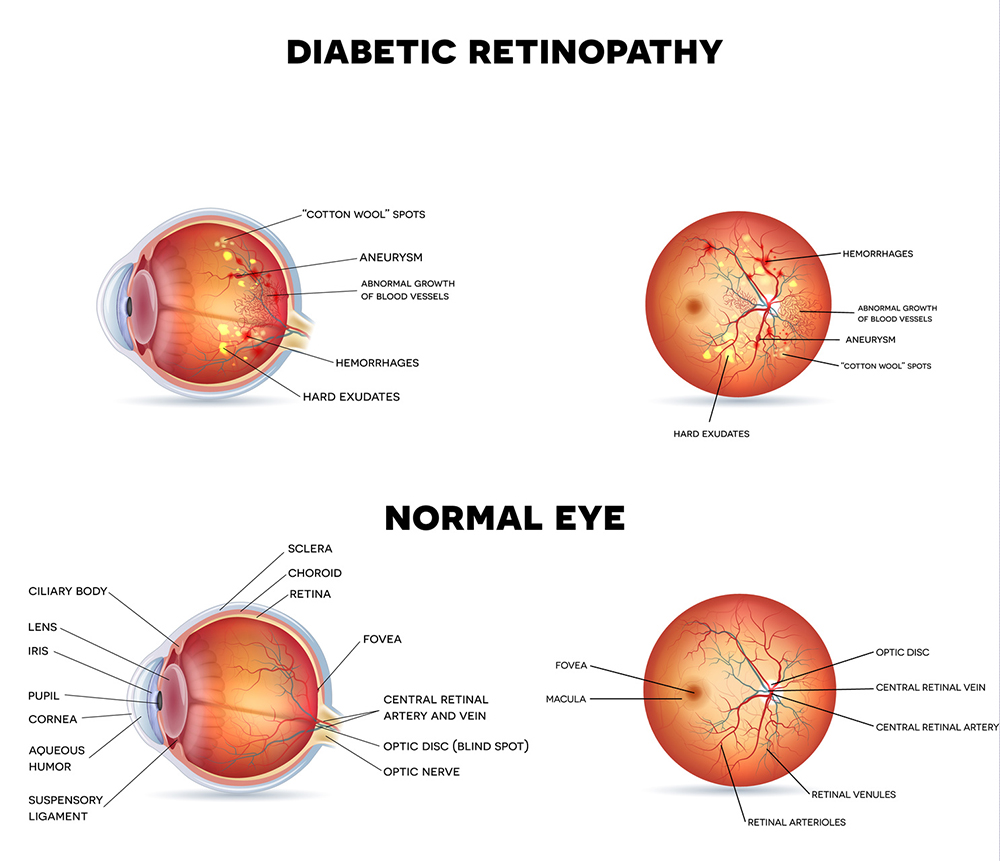
\includegraphics[width=4.16667in,height=3.125in]{images/image 1.jpg}
\caption{Normal Retina Vs Diabetic Retinopathy Retina
(\protect\hyperlink{ref-diabetica}{{``Diabetic Retinopathy Vs Normal,''}
n.d.})}
\end{figure}

\hypertarget{data-pre-processing}{%
\subsection{\texorpdfstring{\emph{Data
pre-processing}}{Data pre-processing}}\label{data-pre-processing}}

Image pre-processing was performed with the aim to decrease unclear
image and reduce image size. The plot below illustrates the class
imbalance in the original dataset.

\begin{figure}
\centering
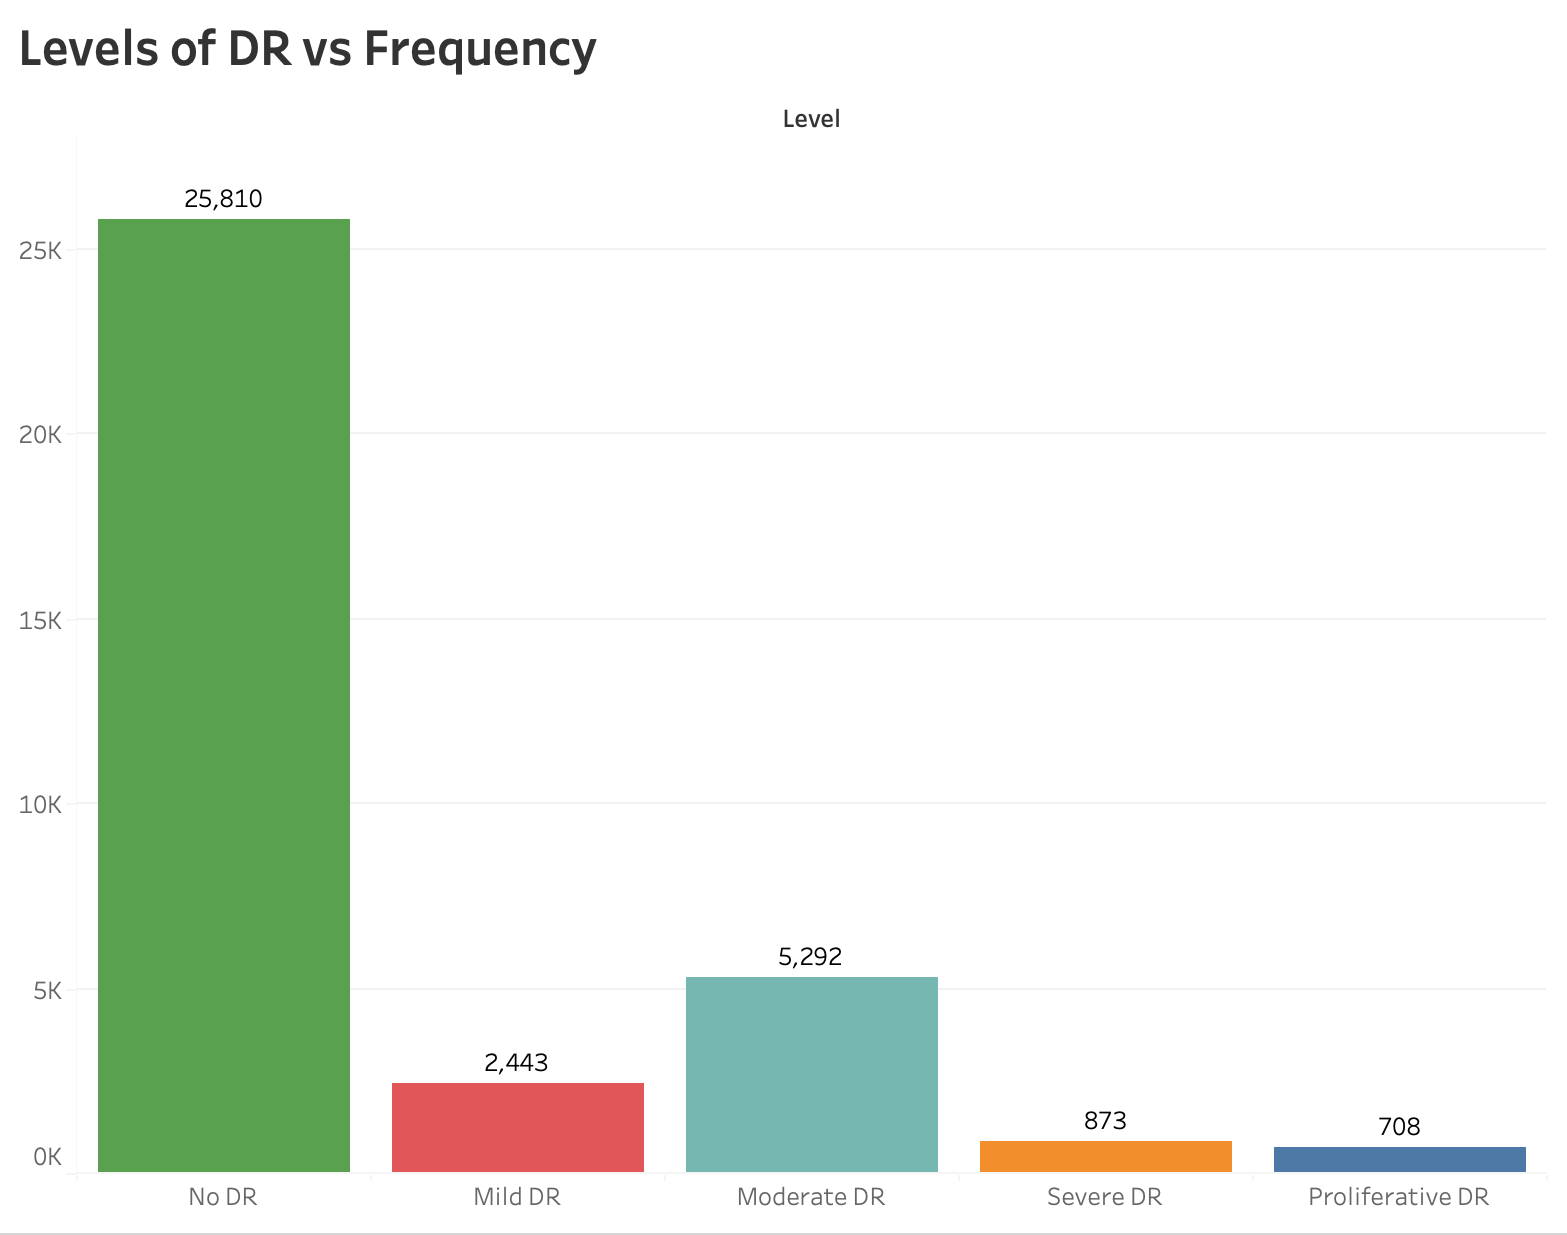
\includegraphics[width=3.57292in,height=\textheight]{images/LevelsOfDR.png}
\caption{Sum of number of records for each level}
\end{figure}

The dataset consist of 35,126 set of images. The orginal image have 1944
* 2592 * 3 size, and all images are jpeg format. The classes have an
uneven distribution of images.

\pagebreak

\begin{enumerate}
\def\labelenumi{\arabic{enumi}.}
\item
  Image Resizing

  Due to the enormous size of the dataset, it was drastically downsized
  before being sent to the network. Each input image is 256 * 256 in
  size after resizing.
\item
  Removing Unclear Image

  Some images have a blackish or white tint. Because it might affect the
  outcome, this type of image cannot be fed into the network. The
  removal of an unclear image is a crucial step that must be taken.
\item
  Dividing images into classes

  Images are classified into 5 folders based on the DR levels.
\end{enumerate}

\pagebreak

\hypertarget{requirements}{%
\section{Requirements}\label{requirements}}

\hypertarget{analysis}{%
\section{Analysis}\label{analysis}}

\hypertarget{design}{%
\section{Design}\label{design}}

\hypertarget{implementation}{%
\section{Implementation}\label{implementation}}

\hypertarget{testing}{%
\section{Testing}\label{testing}}

\hypertarget{project-management}{%
\section{Project Management}\label{project-management}}

\hypertarget{project-schedule}{%
\subsection{Project Schedule}\label{project-schedule}}

\hypertarget{risk-management}{%
\subsection{Risk Management}\label{risk-management}}

\hypertarget{quality-management}{%
\subsection{Quality Management}\label{quality-management}}

\hypertarget{social-legal-ethical-and-professional-considerations}{%
\subsection{Social, Legal, Ethical and Professional
Considerations}\label{social-legal-ethical-and-professional-considerations}}

\hypertarget{critical-appraisal}{%
\section{Critical Appraisal}\label{critical-appraisal}}

\hypertarget{conclusions}{%
\section{Conclusions}\label{conclusions}}

\hypertarget{achievements}{%
\subsection{Achievements}\label{achievements}}

\hypertarget{future-work}{%
\subsection{Future Work}\label{future-work}}

\hypertarget{student-reflections}{%
\section{Student Reflections}\label{student-reflections}}

\newpage

\hypertarget{references}{%
\section{References}\label{references}}

\hypertarget{refs}{}
\begin{CSLReferences}{1}{0}
\leavevmode\vadjust pre{\hypertarget{ref-diabetic2017}{}}%
{``Diabetic Retinopathy - Stages.''} 2017.
\url{https://www.nhs.uk/conditions/diabetic-retinopathy/stages/}.

\leavevmode\vadjust pre{\hypertarget{ref-diabetica_data}{}}%
{``Diabetic Retinopathy Detection.''} 2015.
\url{https://kaggle.com/competitions/diabetic-retinopathy-detection}.

\leavevmode\vadjust pre{\hypertarget{ref-diabetica}{}}%
{``Diabetic Retinopathy Vs Normal.''} n.d.
\url{https://www.advancedretinaassociates.com/patient-education/diabetic-retinopathy/}.

\leavevmode\vadjust pre{\hypertarget{ref-9215270}{}}%
Jayakumari, C., Vidhya Lavanya, and E P Sumesh. 2020. {``Automated
Diabetic Retinopathy Detection and Classification Using ImageNet
Convolution Neural Network Using Fundus Images.''} In \emph{2020
International Conference on Smart Electronics and Communication
(ICOSEC)}, 577--82.
\url{https://doi.org/10.1109/ICOSEC49089.2020.9215270}.

\leavevmode\vadjust pre{\hypertarget{ref-9828576}{}}%
Kaya, Esra, and Ismail Saritas. 2022. {``Performances of CNN
Architectures on Diabetic Retinopathy Detection Using Transfer
Learning.''} In \emph{2022 57th International Scientific Conference on
Information, Communication and Energy Systems and Technologies (ICEST)},
1--4. \url{https://doi.org/10.1109/ICEST55168.2022.9828576}.

\leavevmode\vadjust pre{\hypertarget{ref-9651024}{}}%
Kumar, Nikhil Sathya, and B. Ramaswamy Karthikeyan. 2021. {``Diabetic
Retinopathy Detection Using CNN, Transformer and MLP Based
Architectures.''} In \emph{2021 International Symposium on Intelligent
Signal Processing and Communication Systems (ISPACS)}, 1--2.
\url{https://doi.org/10.1109/ISPACS51563.2021.9651024}.

\leavevmode\vadjust pre{\hypertarget{ref-pratt2016convolutional}{}}%
Pratt, Harry, Frans Coenen, Deborah M Broadbent, Simon P Harding, and
Yalin Zheng. 2016. {``Convolutional Neural Networks for Diabetic
Retinopathy.''} \emph{Procedia Computer Science} 90: 200--205.

\leavevmode\vadjust pre{\hypertarget{ref-r2015}{}}%
R, Lee, Wong Ty, and Sabanayagam C. 2015. {``Epidemiology of Diabetic
Retinopathy, Diabetic Macular Edema and Related Vision Loss.''}
\emph{Eye and Vision (London, England)} 2 (September).
\url{https://doi.org/10.1186/s40662-015-0026-2}.

\end{CSLReferences}

\newpage

Appendix A -- Project Specification

Appendix B -- Interim Progress Report and Meeting Records

Appendix C -- Requirements Specification Document

Appendix D -- User Manual

Appendix E -- Project Presentation

Appendix F -- Certificate of Ethics Approval

\end{document}
